\documentclass[]{beamer}

\usepackage{tikz}
\usetikzlibrary{shapes.geometric, arrows}
\tikzstyle{result} = [rectangle, rounded corners, minimum width=3cm, minimum height=0.5cm, text centered, draw=black, fill=green!30]
\tikzstyle{process} = [rectangle, minimum width=3cm, minimum height=0.5cm, text centered, draw=black, fill=orange!30]
\tikzstyle{arrow}= [thick,->,>=stealth]
\usepackage{movie15}
\usepackage{lipsum}
\usepackage{pgfpages}
\usepackage{graphicx}
\usepackage[dutch]{babel}
\graphicspath{{img/}}

\mode<handout>{%
%	\setbeameroption{show notes}
}

\usetheme{AnnArbor}
\usecolortheme{beaver}

\AtBeginSection[]
{
	\begin{frame}
		\frametitle{Inhoudsopgave}
		\tableofcontents[currentsection]
	\end{frame}
}


\begin{document}
	\title[Actieherkenning met de Kinect sensor]{Intuïtieve mens-machineinterface met live actieherkenning }
	\author[Bert De Saffel]{
				\begin{tabular}{rcr}
				prof. dr. ir. Peter Veelaert &\&& prof. dr. ir. Wilfried Philips \\
				ing. Sanne Roegiers &\&& ing. Dimitri van Cauwelaert
				\end{tabular}
	}
	
	\subtitle{Master of Science in de industriële wetenschappen: informatica \\ \vspace{0.2cm} Bert De Saffel}
	\date{04 april 2019}
	\frame{\titlepage}
	
	\begin{frame}{Inhoudsopgave}
		\begin{enumerate}
			\item Context
			\item Probleemstellingen
			\item Methodologie
		\end{enumerate}
	\end{frame}
	
	\section{Context}

	\begin{frame}{Context}
		\begin{itemize}
			\item Oorzaken van ernstige arbeidsongevallen in 2015
			\begin{enumerate}
				\item Verlies van controle over een machine of voertuig
				\item Uitglijden of struikelen
				\item Het tillen of neerzetten van lasten
				\item Vrijkomen van giftige producten
			\end{enumerate}
			\item<2-> Gevolgen
			\begin{itemize}
				\item Langdurige ongeschiktheid
				\item Permanente letsels
				\item Sterfgeval
			\end{itemize}
		\end{itemize}
	\end{frame}
	\begin{frame}{Context}
		\begin{figure}
			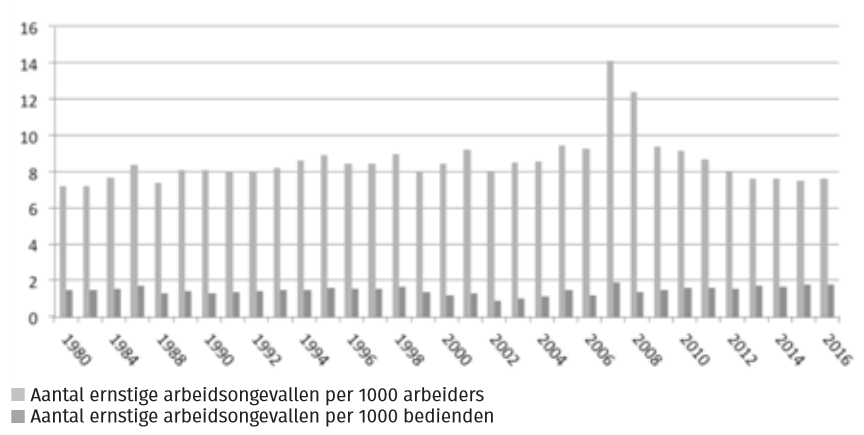
\includegraphics[width=0.7\textwidth]{arbeidsongevallen}
			\caption{Frequentiegraad ernstige arbeidsongevallen in de privésector.}
		\end{figure}
	\end{frame}

	\begin{frame}{Context}
		\begin{itemize}
			\item Mogelijke oplossing
			\begin{itemize}
				\item Het inzetten van robotica in gevaarlijke omgevingen
				\item<2-> Hoe besturen?
				\begin{itemize}
					\item Remote control
					\item Autonoom
					\item Actieherkenning
				\end{itemize}
			\end{itemize}
		\end{itemize}
	\end{frame}

	\begin{frame}\frametitle{Context}
		\begin{itemize}
			\item De verplaatsing van een robot uitvoeren met enkel actieherkenning
			\item<2-> Met de kinect sensor
			\begin{itemize}
				\item Kan skeletbeelden genereren vanuit RGB-D data
			\end{itemize}
			\begin{figure}
				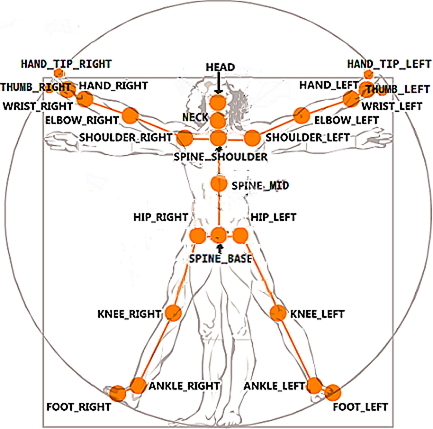
\includegraphics[width=0.4\textwidth]{skeleton}
			\end{figure}	
		\end{itemize}
	\end{frame}

	\section{Probleemstellingen}
	\begin{frame}\frametitle{Probleemstellingen}
		\begin{enumerate}
			\item Verschillen in lichaamsbouw mogelijk (klein vs groot)
			\item Verschillen in camerahoek
			\item<2-> Real-time actieherkenning
			\begin{itemize}
				\item De actie herkennen op het moment dat deze uitgevoerd wordt
			\end{itemize} 
		\end{enumerate}
		\begin{figure}
			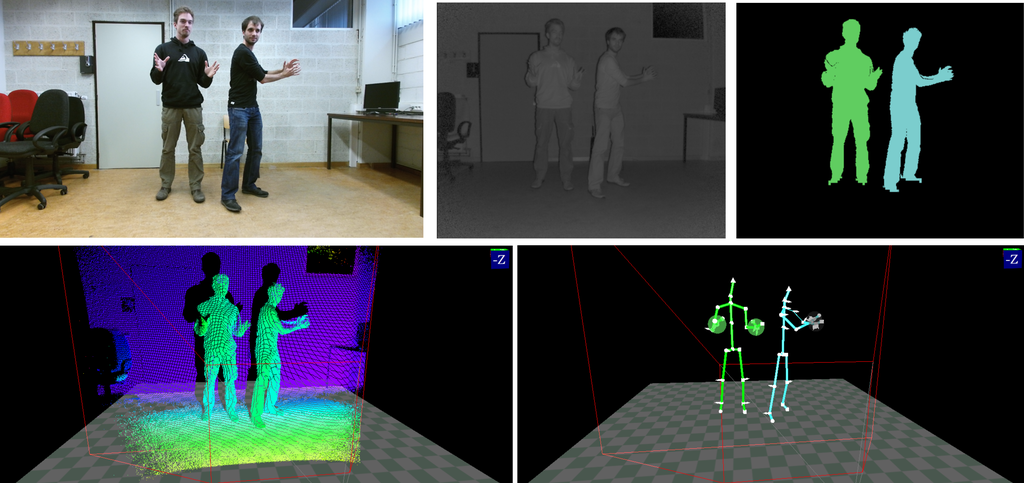
\includegraphics[width=\textwidth]{sensoren}
		\end{figure}
	\end{frame}

	\begin{frame}\frametitle{Onderzoek}
		\begin{enumerate}
			\item De features moeten rotatie- en lichaamsinvariant zijn
			\item Actie moet vroeg genoeg herkend worden om live te kunnen classificeren
		\end{enumerate}
	\end{frame}


	\section{Methodologie}
	\subsection{Machine Learning}
	\begin{frame}{Machine Learning - Classificatieprobleem}
			\begin{itemize}
				\item Een verzameling van klassen (labels, uitvoerwaarden, ...)
				\item \textbf{Gegeven een observatie, tot welke klasse behoort deze observatie?}
				\item Bij actieherkenning:
				\begin{itemize}
					\item Klassen = acties
					\item Observaties = frames
				\end{itemize}
			\end{itemize}

	\end{frame}
	
	\begin{frame}{Machine Learning - Features}
		\begin{itemize}
			\item Een observatie (frame) wordt getransformeerd naar \textit{features}
			\begin{itemize}
				\item Pixel: RGB-waarden
				\item Persoon: leeftijd, geslacht, haarkleur, lengte, ...
			\end{itemize}
			\item Features op basis van skeletbeelden
			\begin{itemize}
				\item Elk skelet \textit{joint} wordt gekenmerkt door zijn ($x, y, z$) coördinaten
				\item Het skelet bestaat uit 25 \textit{joints}
				\item[$\rightarrow$] 75-dimensionale \textit{feature vector}
				
				$$\textbf{f} = \begin{pmatrix}
				x_1 & y_1 & z_1 & ...&  x_{25} & y_{25} & z_{25}
				\end{pmatrix}$$
			\end{itemize}
		\end{itemize}
		
	\end{frame}

	\begin{frame}{Machine Learning - Classificatie}
		
	\end{frame}
	\subsection{Dataset}
	\begin{frame}{Dataset}
		content...
	\end{frame}
	\subsection{Preprocessing}
	\begin{frame}{Preprocessing}
		\begin{enumerate}
			\item[1.]<1-> Plaats-invariantie $\rightarrow$ Translatie
			\begin{itemize}
				\item \textit{Spine base joint} als oorsprong:
				$$\begin{pmatrix}
				x' \\
				y' \\
				z'
				\end{pmatrix}
				= \begin{pmatrix}
				x \\ y \\ z
				\end{pmatrix}
				- \begin{pmatrix}
				x_0 \\ y_0 \\ z_0
				\end{pmatrix}$$
				met $x_0, y_0, z_0$ de drie-dimensionale coördinaten van de \textit{Spine base joint}
			\end{itemize}
			\item[2.]<2-> Schaal-invariantie $\rightarrow$ Vectornormalisatie 
			\begin{itemize}
				\item Elk component van elke positievector delen door lengte van de \textit{neck joint} positievector:
				$$
				\begin{pmatrix}
				x' \\ y' \\ z'
				\end{pmatrix}
				=				
				\begin{pmatrix}
				\frac{x}{||n||} \\ \frac{y}{||n||}  \\ \frac{z}{||n||} 
				\end{pmatrix}
				$$
				met $$||n|| = \sqrt{(neck_x)^2 + (neck_y)^2 + (neck_z)^2}$$
			\end{itemize}
		\end{enumerate}
	\end{frame}

	\begin{frame}
		\begin{enumerate}
			\item[3.]<1-> Rotatie-invariantie $\rightarrow$ Lokaal skeletcoördinatensysteem $(X', Y', Z')$
			\begin{itemize}
				\item X'-as = de as door de 
				\item Y'-as = de as door de 
				\item Z'-as = orthogonaal met X' en Y'
				\item Via quaternionen:
				$$\textbf{q} = a + b\textbf{i} + c\textbf{j} + d\textbf{k}$$
				\begin{itemize}
					\item Vierdimensionale uitbreiding van de reële getallen
					\item $b\textbf{i} + c\textbf{j} + d\textbf{k}$ is drie-dimensionaal en reflecteerd de ruimte $R^3$.
						\item Sneller en compacter dan drie-dimensionale rotatiematrices
					\item Rotatie rond $x-as$:
					$$
						\hbox{bgtg}\bigg(\frac{2ab + 2cd}{1 - 2b^2 + 2c^2}\bigg)\qquad \hbox{radialen}
					$$

				
				\end{itemize}

				
			\end{itemize}
	\end{enumerate}
	\end{frame}
	\begin{frame}{Preprocessing}
	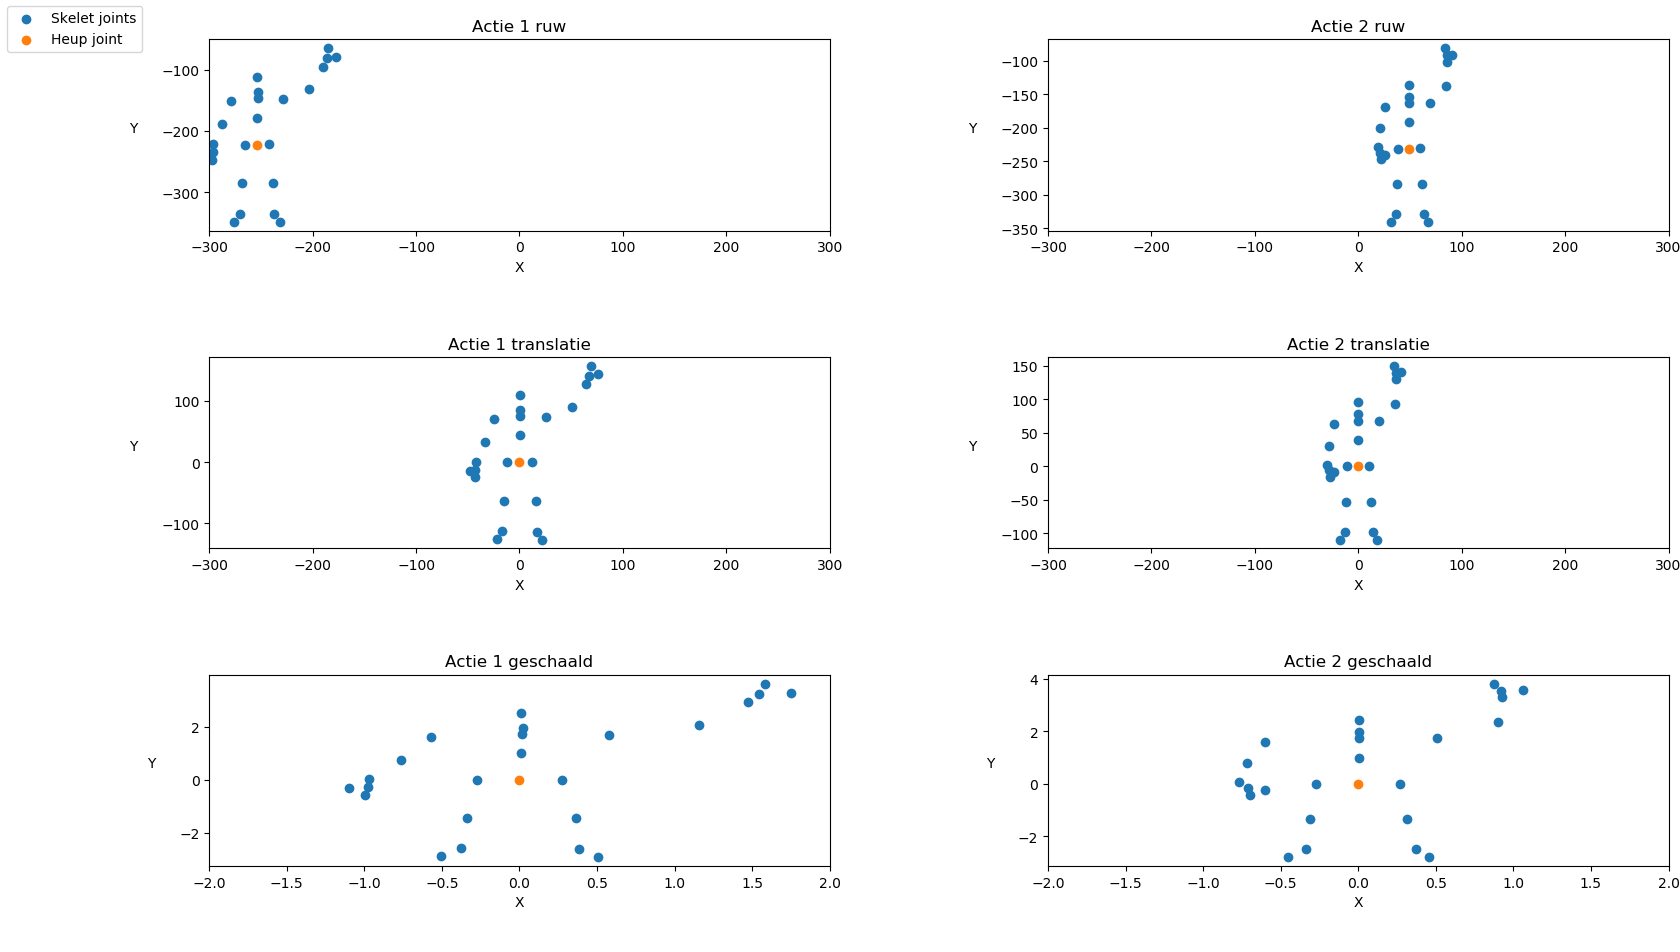
\includegraphics[width=\textwidth]{skeleton_preprocessing}
	\end{frame}
	
	\subsection{Feature transformatie}
	
	\subsection{Classificatie}
	\begin{frame}
		\begin{itemize}
			\item 
		\end{itemize}
	\end{frame}
	\subsection{Evaluatie}
	\begin{frame}{Evaluatie}
		\begin{itemize}
			\item Confusion matrix
			\begin{figure}[ht]
				\centering
				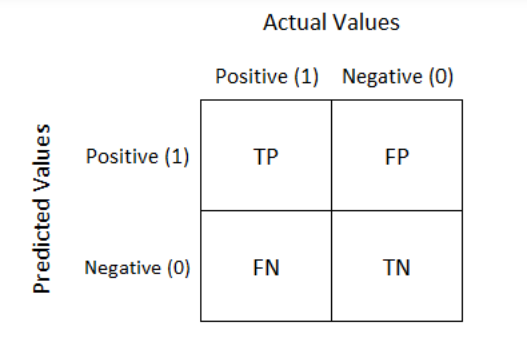
\includegraphics[width=0.5\textwidth]{confusionmatrix}
			\end{figure}
		
				\item Precision = $\frac{TP}{TP + FP}$
				\item Recall = $\frac{TP}{TP + FN}$
				\item F1 score = $2*\frac{precision * recall}{precision + recall}$
		
		\end{itemize}
	\end{frame}
	\begin{frame}{Evaluatie}
		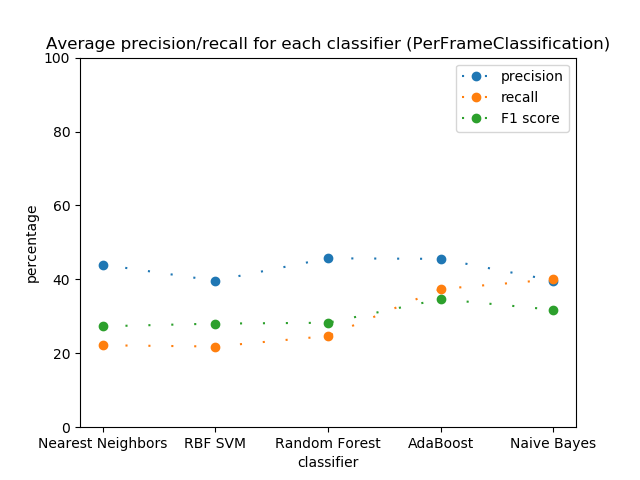
\includegraphics[width=0.5\textwidth]{PerFrameClassification_PreProcessing}
		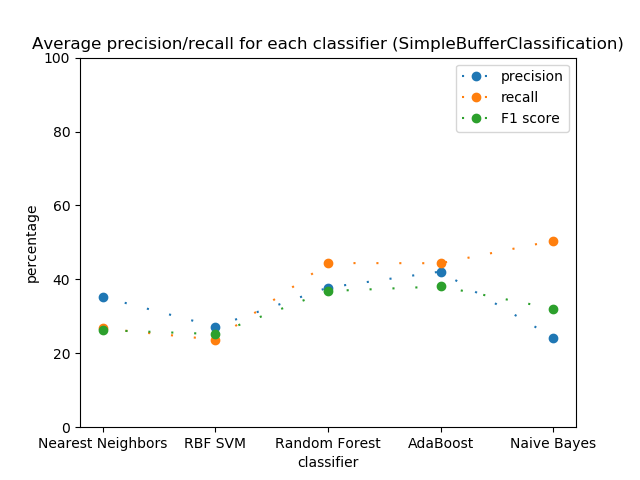
\includegraphics[width=0.5\textwidth]{SimpleBufferClassification_PreProcessing}
	\end{frame}
	
	
	\begin{frame}
		\begin{center}
			\Huge Vragen, opmerkingen, ...?
		\end{center}
	\end{frame}
\end{document}